\section{Results}

\subsection{Quality evaluation}

The RNA-seq data was initially assessed with FastQC\index{FastQC}, and according to this assessment the data was preprocessed/trimmed with Trimmomatic\index{Trimmomatic} and afterwards assessed again with FastQC (see section \ref{RNA-seq-preprocessing}). Finally, an overall report on the data preprocessing, the quality assessments and the kallisto\index{kallisto} pseudoalignments was created with MultiQC\index{MultiQC}.

Figure \ref{fig:0.1-MultiQC_FastQC_status_checks} shows the MultiQC report on the Trimmomatic\index{Trimmomatic} preprocessing (the surviving reads).

\begin{figure}[htbp]
    \caption{Trimmomatic preprocessing}
    \label{fig:0.1-MultiQC_FastQC_status_checks}
    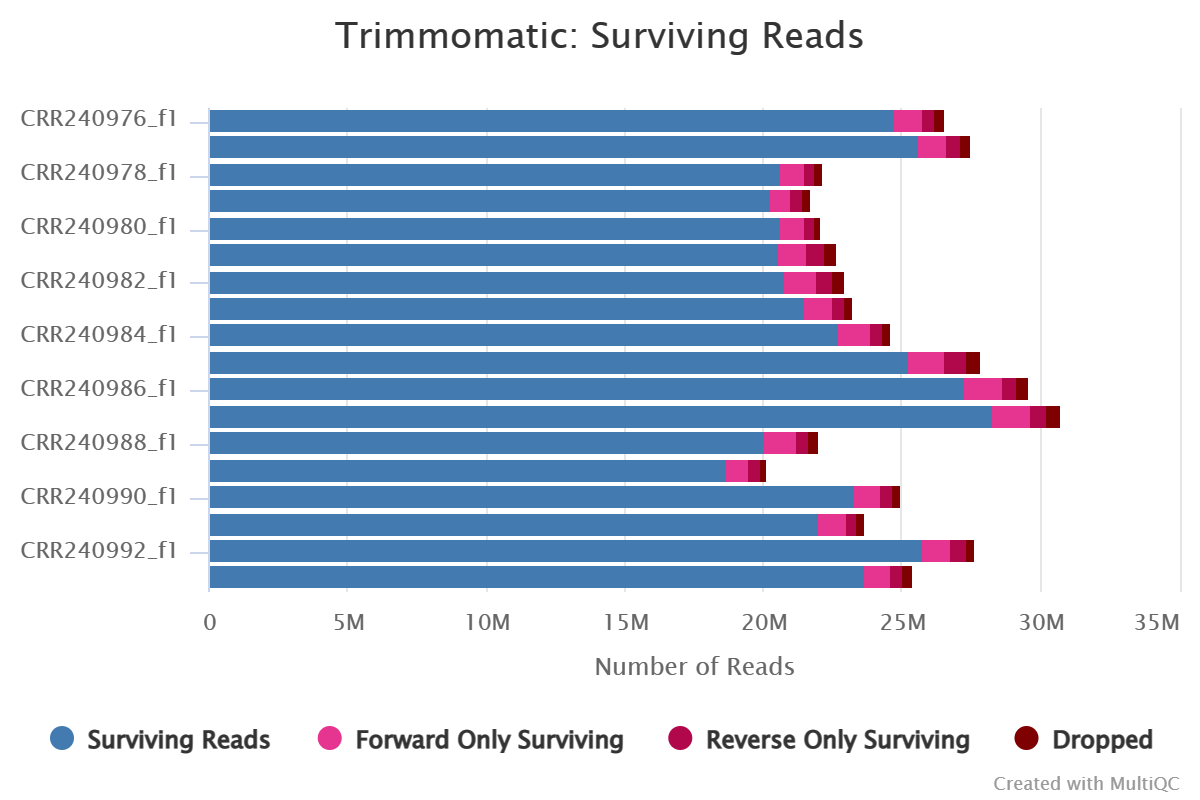
\includegraphics[width=0.75\textwidth]{../../results/multiqc/Plot-Exports/trimmomatic-surviving_reads}
\end{figure}

Figure \ref{fig:0.2-MultiQC_FastQC_status_checks} shows the MultiQC overview of the FastQC\index{FastQC} quality assessments of the trimmed FASTQ files.

\begin{figure}[htbp]
    \caption{FastQC quality assessment of the preprocessed FASTQ files}
    \label{fig:0.2-MultiQC_FastQC_status_checks}
    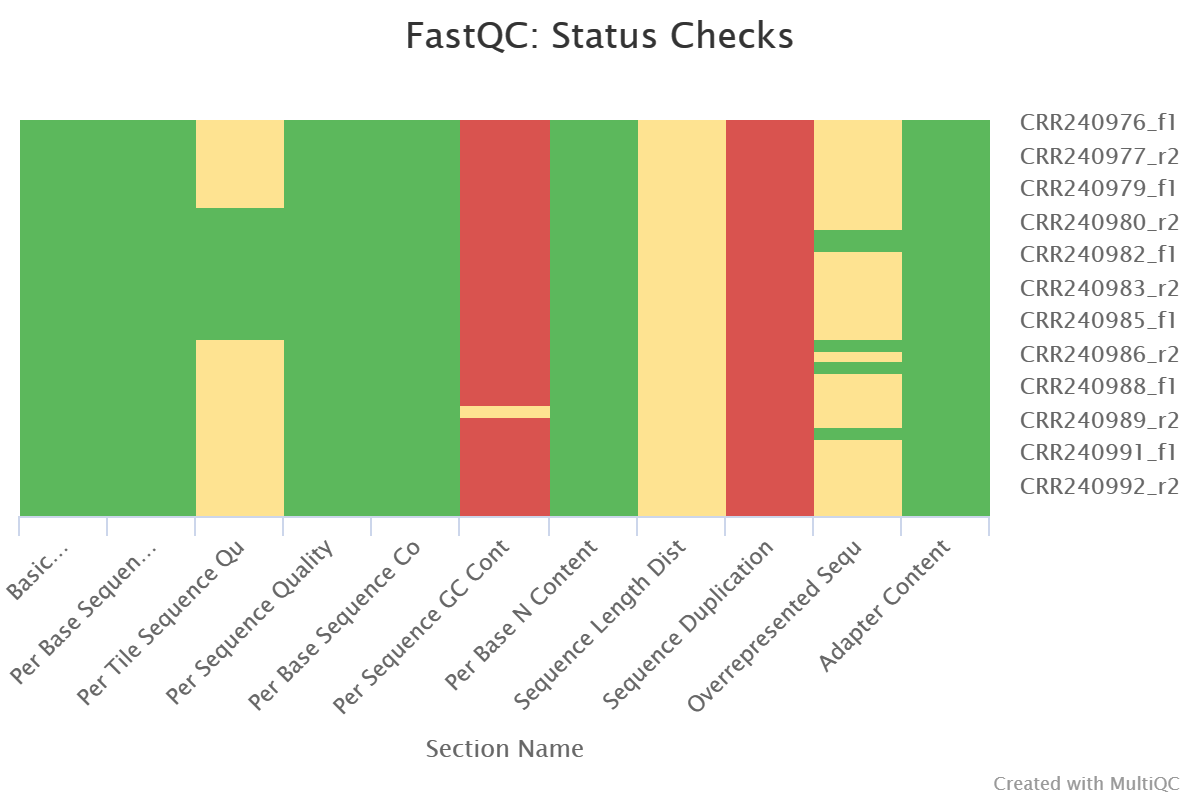
\includegraphics[width=0.75\textwidth]{../../results/multiqc/Plot-Exports/fastqc-status-check-heatmap}
\end{figure}

According to these quality assessments, the (trimmed) RNA-seq data may be regarded as good quality for the purpose of this research.


\subsection{Reads mapped to the reference transcriptome}

For most of the FASTQ files, kallisto pseudoaligned well above 80 \% of the (preprocessed) RNA-seq reads. Figure \ref{fig:0.3-MultiQC_kallisto_alignment} shows a MultiQC overview of the kallisto\index{kallisto} pseudoalignments.

\begin{figure}[htbp]
    \caption{kallisto pseudoalignments}
    \label{fig:0.3-MultiQC_kallisto_alignment}
    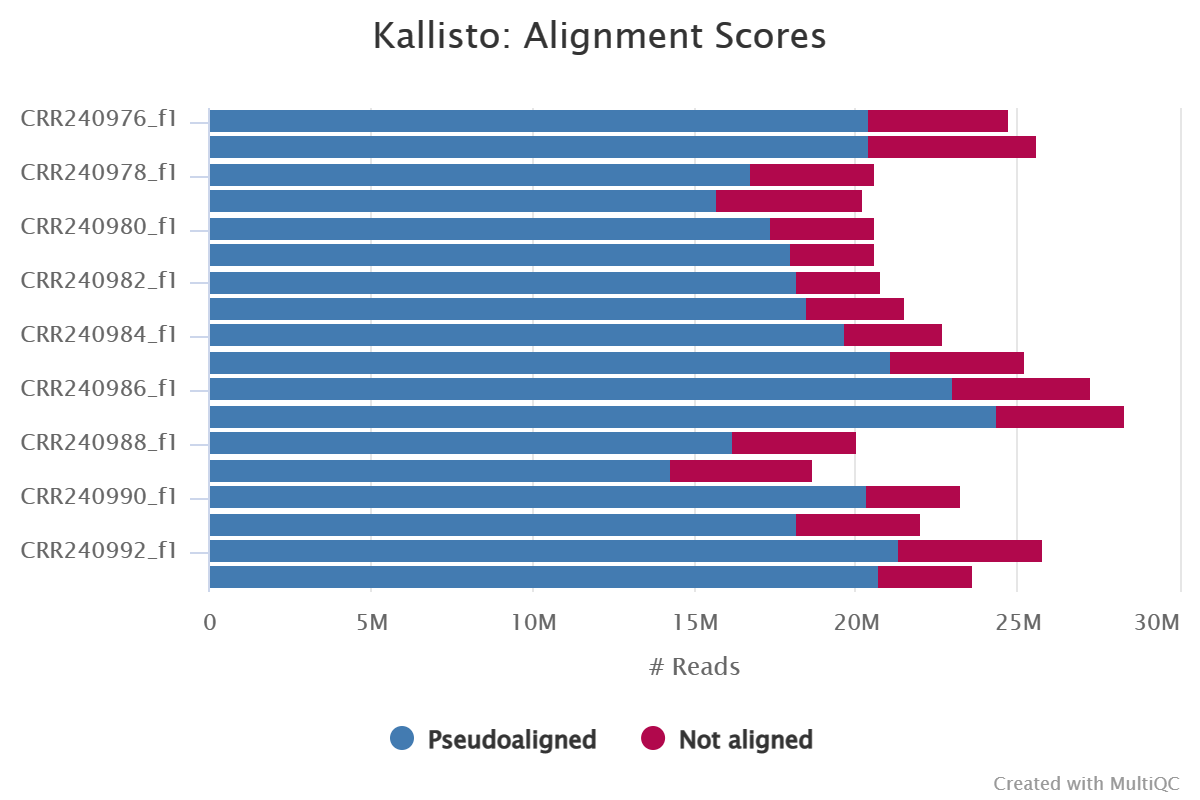
\includegraphics[width=0.75\textwidth]{../../results/multiqc/Plot-Exports/kallisto_alignment}
\end{figure}


\subsection{Hierarchical cluster analysis}

The hierarchical cluster analysis \index{hierarchical cluster analysis (HCA)} (see section \ref{hierarchical-cluster-analysis}) reveals that the normal condition groups and the drought stress condition groups are closely related (grouped together). But the data for O. nivara also shows that the cultivar has an even greater impact on the clustering then the drought stress condition (see figures \ref{fig:3.1-Clust-Dendrogram-Oryza_nivara} and \ref{fig:3.1-Clust-Dendrogram-Oryza_sativa}).

\begin{figure}[htbp]
    \caption{Hierarchical cluster analysis of the O. nivara RNA-seq data}
    \label{fig:3.1-Clust-Dendrogram-Oryza_nivara}
    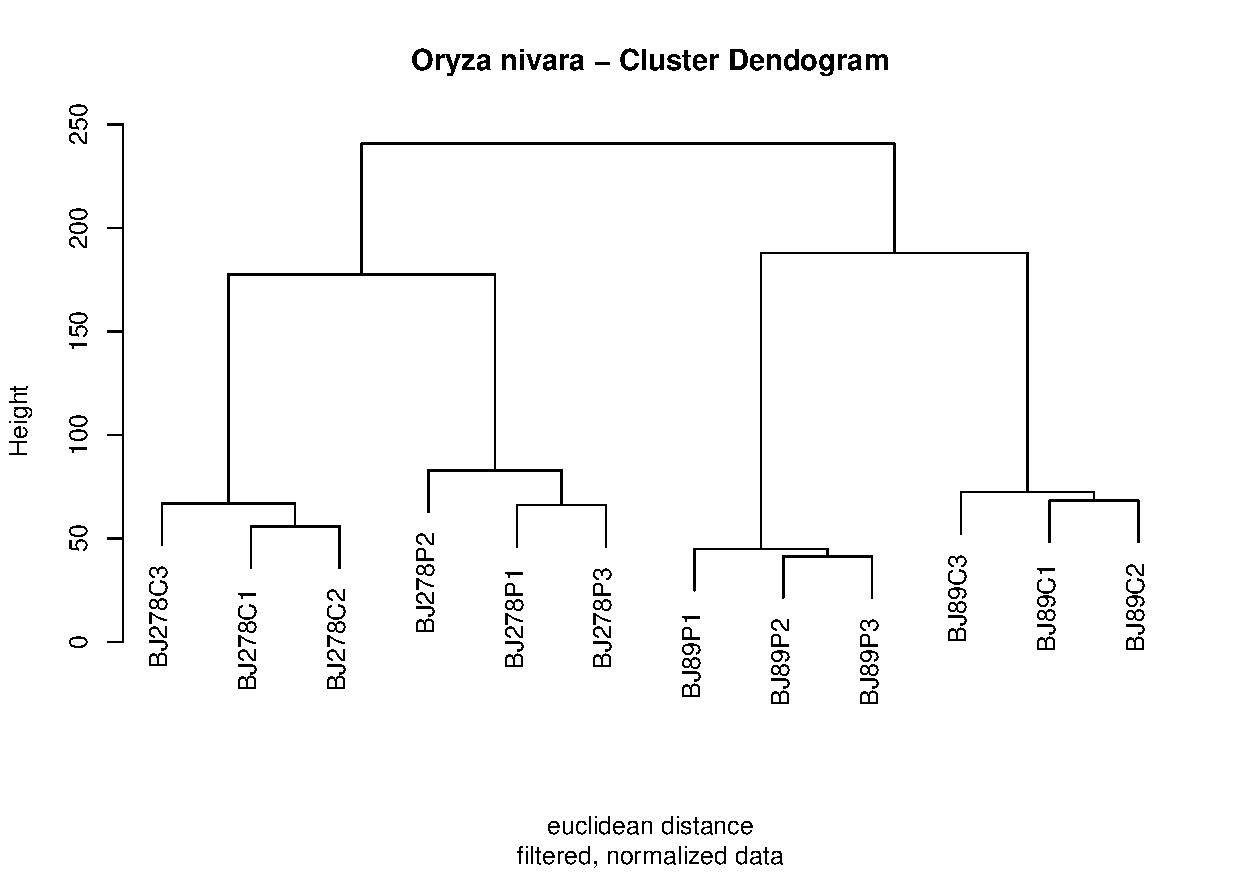
\includegraphics[width=0.75\textwidth]{../../results/plots-and-tables/3.1-Clust-Dendrogram-Oryza_nivara}
\end{figure}

\begin{figure}[htbp]
    \caption{Hierarchical cluster analysis of the O. sativa RNA-seq data}
    \label{fig:3.1-Clust-Dendrogram-Oryza_sativa}
    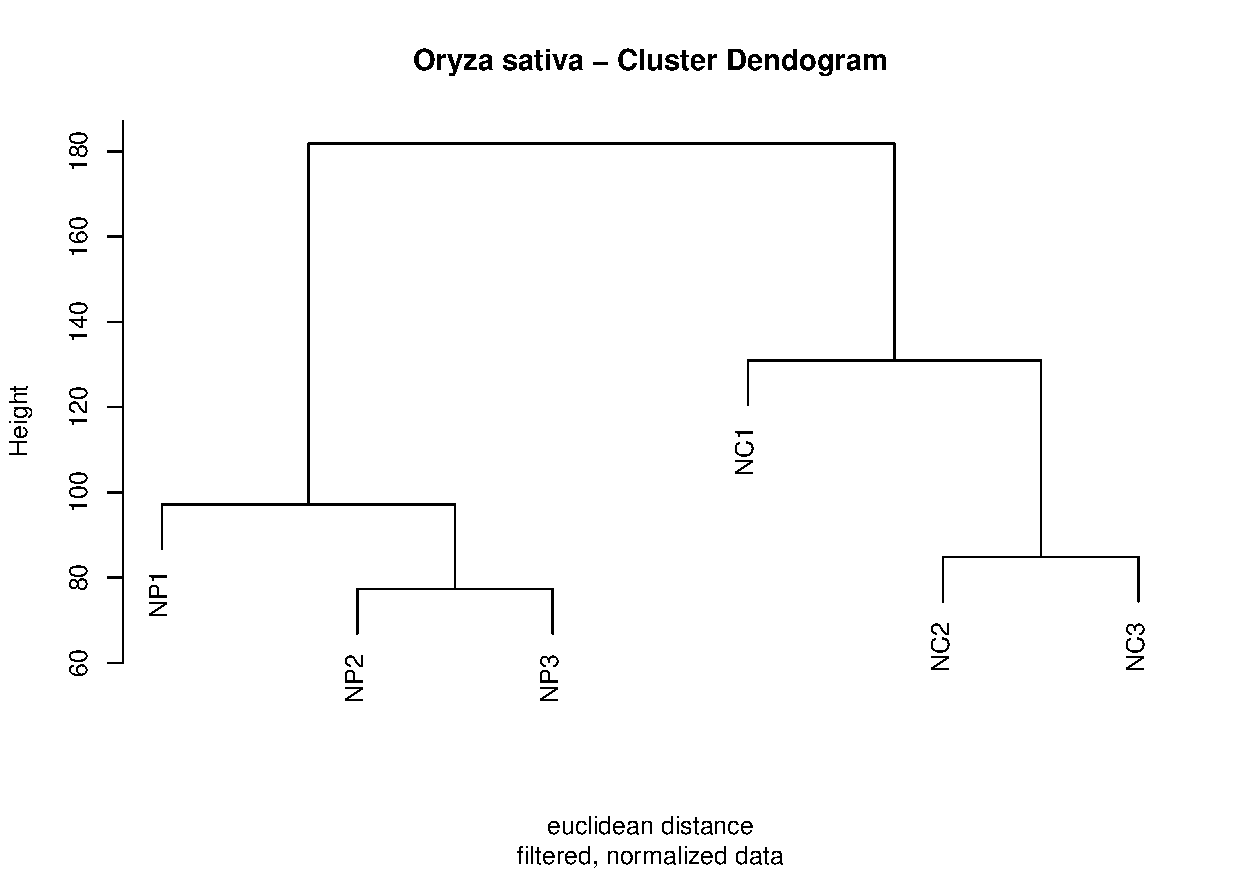
\includegraphics[width=0.75\textwidth]{../../results/plots-and-tables/3.1-Clust-Dendrogram-Oryza_sativa}
\end{figure}


\subsection{Principal component analysis}

The principal component analysis (PCA)\index{principal component analysis (PCA)} (see section \ref{principal-component-analysis}) reveals that for both O. nivara and O. sativa the first two principal components account for more than 80 \% of the variance in the gene expression. Figures  \ref{fig:3.2-PCA-Oryza_nivara} and \ref{fig:3.2-PCA-Oryza_sativa} show the contribution percentage of the samples to the first two principal components (PCs)\index{principal component analysis (PCA)!principal component (PC)} for the two species.

For O. nivara, the samples from the same condition (normal vs drought stress) cluster together, with a tight clustering of the two different cultivars. This means that the different conditions might well explain the differences in gene expression, with the cultivar being an important confounding factor.

For O. sativa, the samples from the same condition cluster together with the exception of sample "NC1". This might be due to a batch effect\index{batch effect}.

\begin{figure}[htbp]
    \caption{PCA of the log2(CPM) data - O. nivara}
    \label{fig:3.2-PCA-Oryza_nivara}
    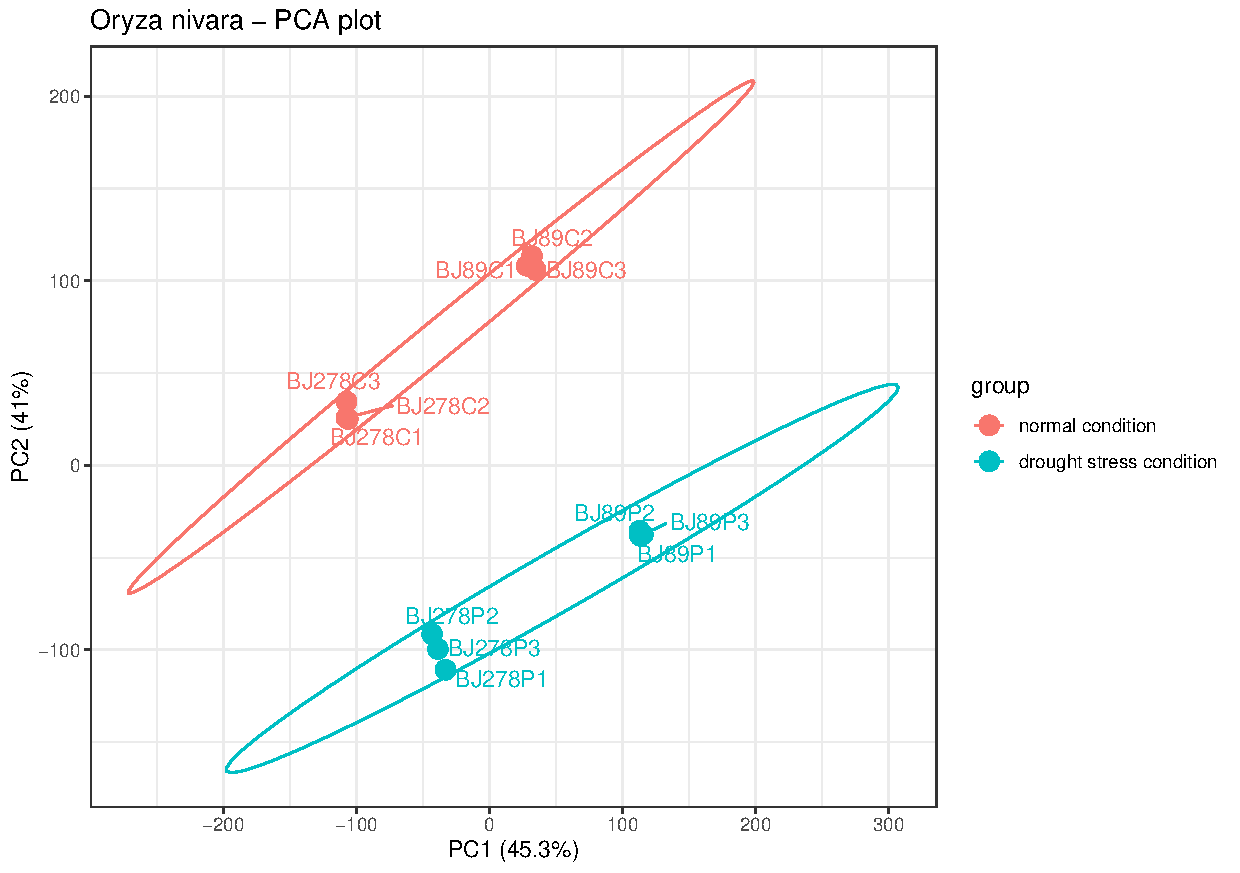
\includegraphics[width=0.75\textwidth]{../../results/plots-and-tables/3.2-PCA-Oryza_nivara}
\end{figure}

\begin{figure}[htbp]
    \caption{PCA of the log2(CPM) data - O. sativa}
    \label{fig:3.2-PCA-Oryza_sativa}
    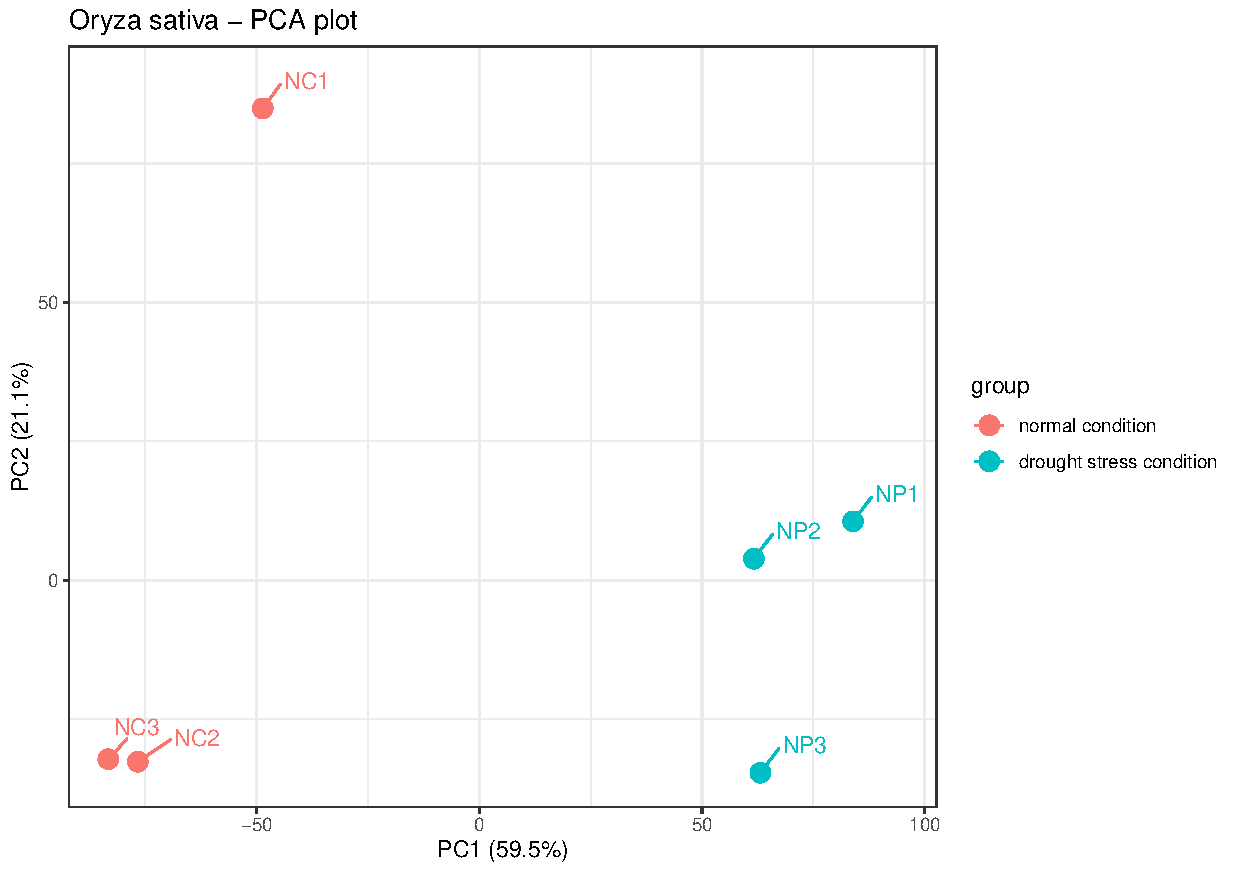
\includegraphics[width=0.75\textwidth]{../../results/plots-and-tables/3.2-PCA-Oryza_sativa}
\end{figure}


\subsection{Differentially expressed genes}



\begin{figure}[htbp]
    \caption{Volcano plot of the DEGs - O. nivara}
    \label{fig:4.1-DEG-Volcano-Plot-Oryza_nivara}
    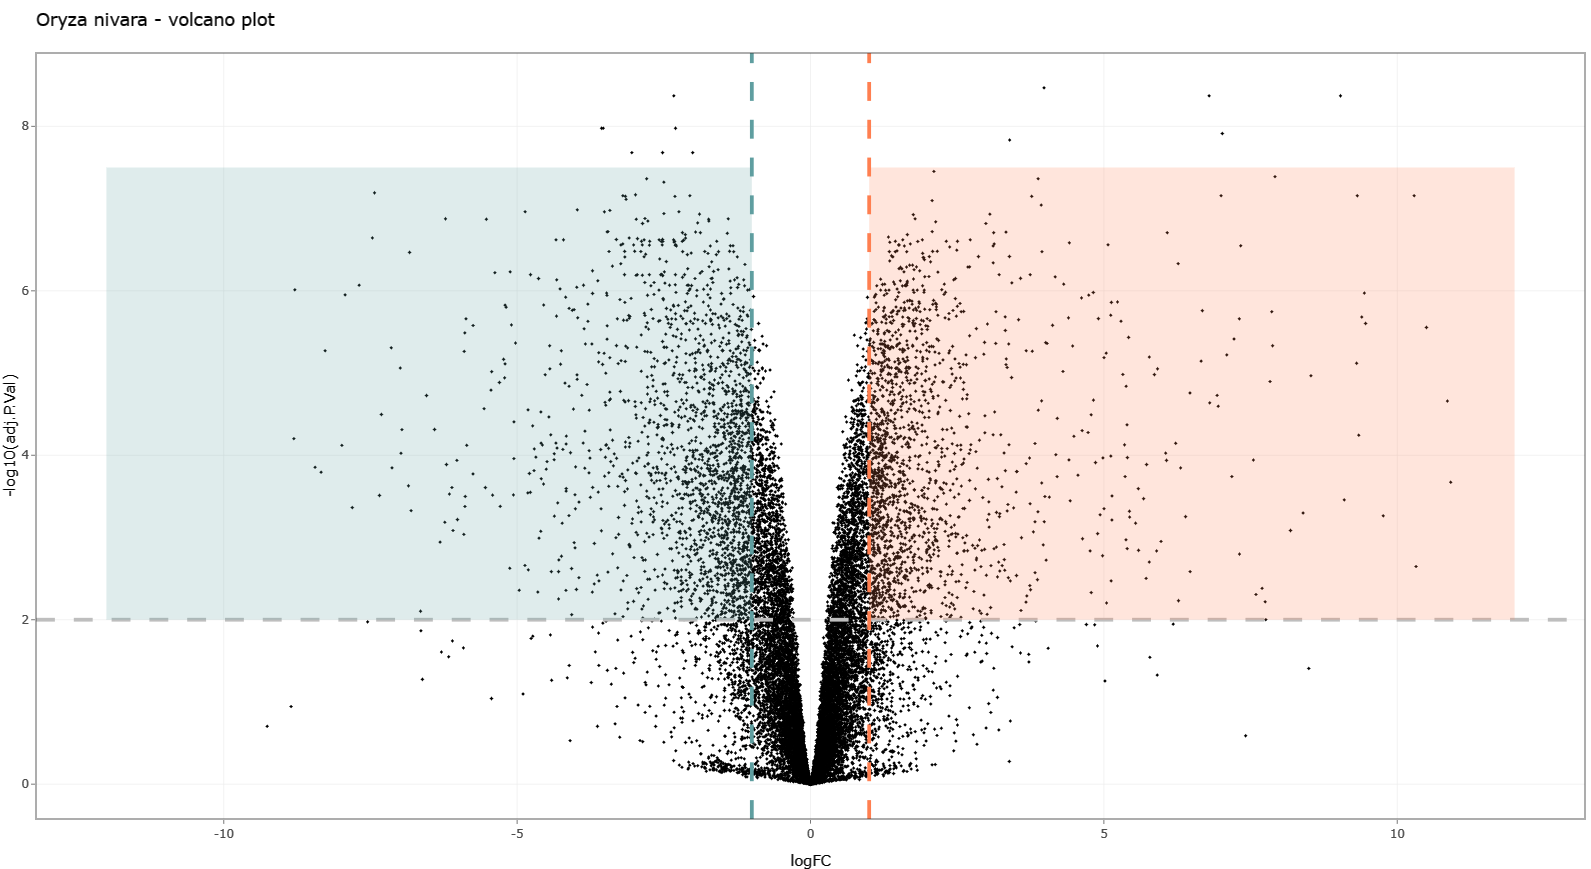
\includegraphics[width=\textwidth]{../../results/plots-and-tables/4.1-DEG-Volcano-Plot-Oryza_nivara}
\end{figure}

\begin{figure}[htbp]
    \caption{Volcano plot of the DEGs - O. sativa}
    \label{fig:4.1-DEG-Volcano-Plot-Oryza_sativa}
    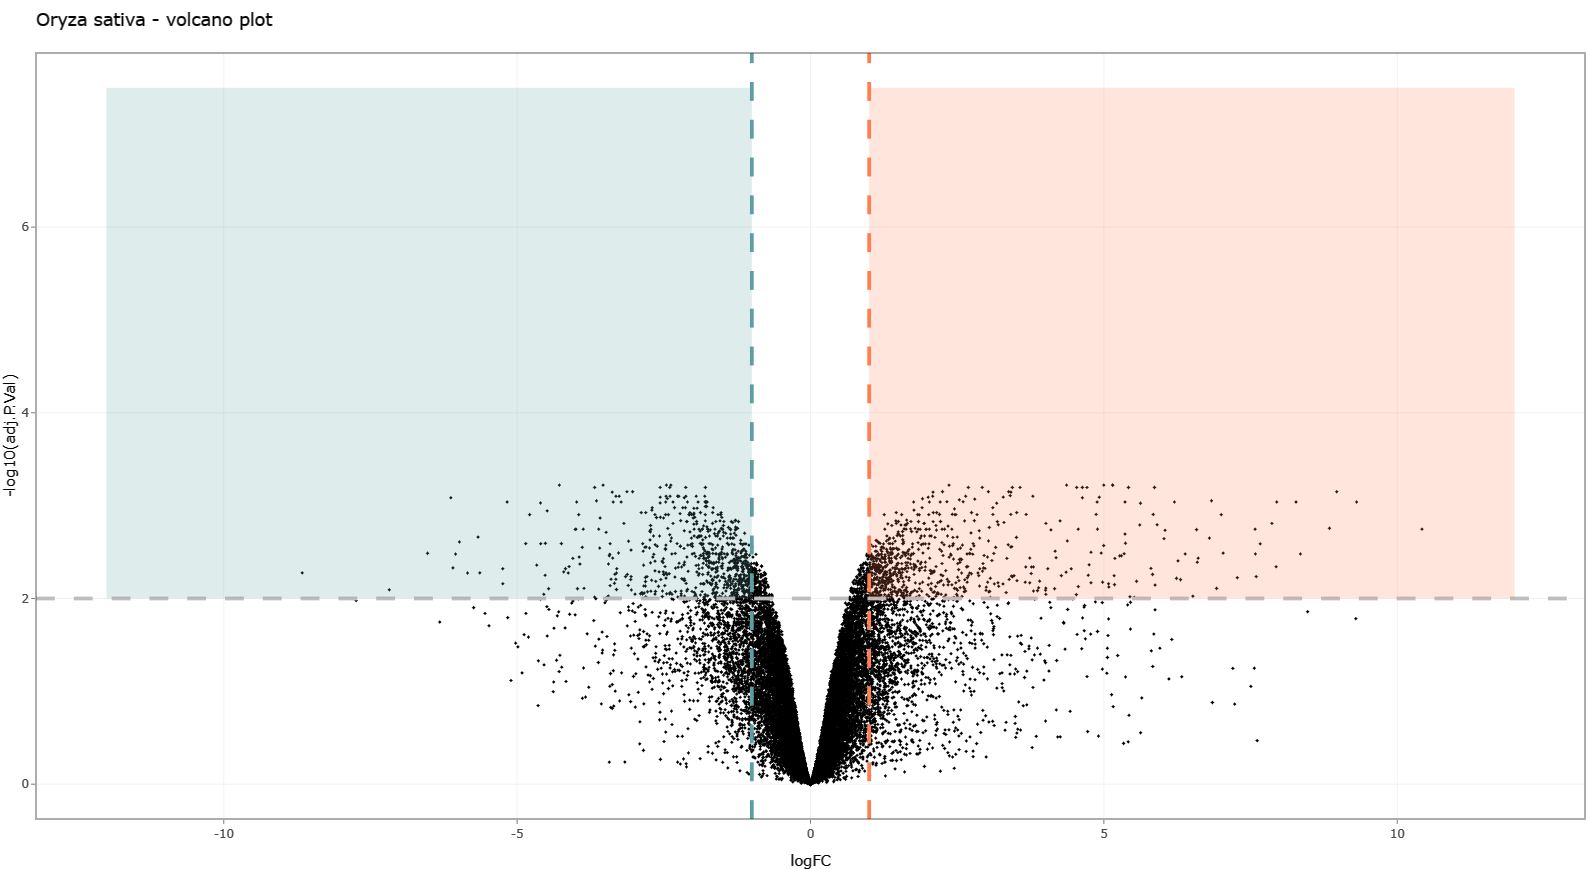
\includegraphics[width=\textwidth]{../../results/plots-and-tables/4.1-DEG-Volcano-Plot-Oryza_sativa}
\end{figure}



\begin{figure}[htbp]
    \caption{Venn diagrams of the DEGs}
    \label{fig:4.2-DEG-Venn-Diagr}
    \begin{subfigure}[t]{0.48\linewidth}
        \caption{O. nivara}
        \label{fig:4.2-DEG-Venn-Diagr-Oryza_nivara}
        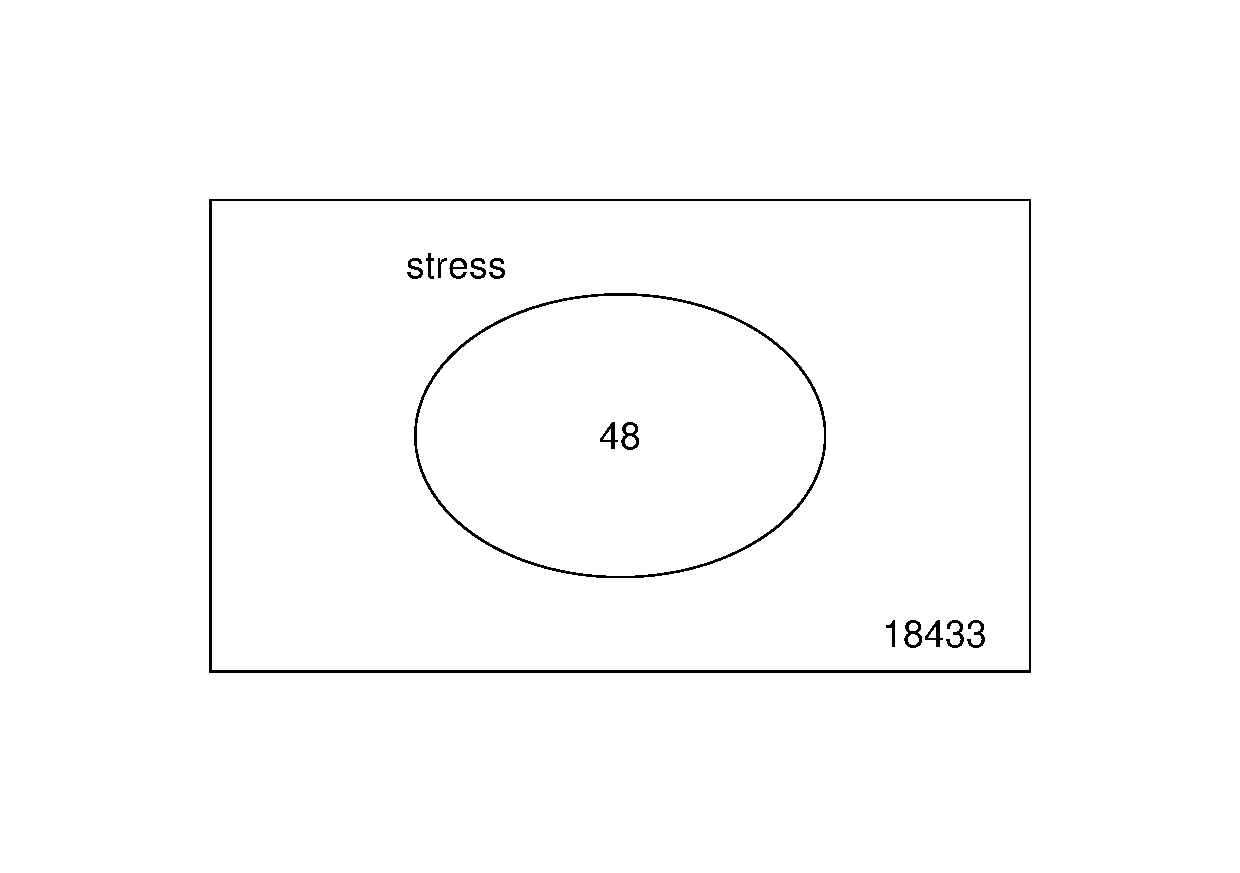
\includegraphics[width=\textwidth, height=4cm]{../../results/plots-and-tables/4.2-DEG-Venn-Diagr-Oryza_nivara}
    \end{subfigure}
    \begin{subfigure}[t]{0.48\linewidth}
        \caption{O. sativa}
        \label{fig:4.2-DEG-Venn-Diagr-Oryza_sativa}
        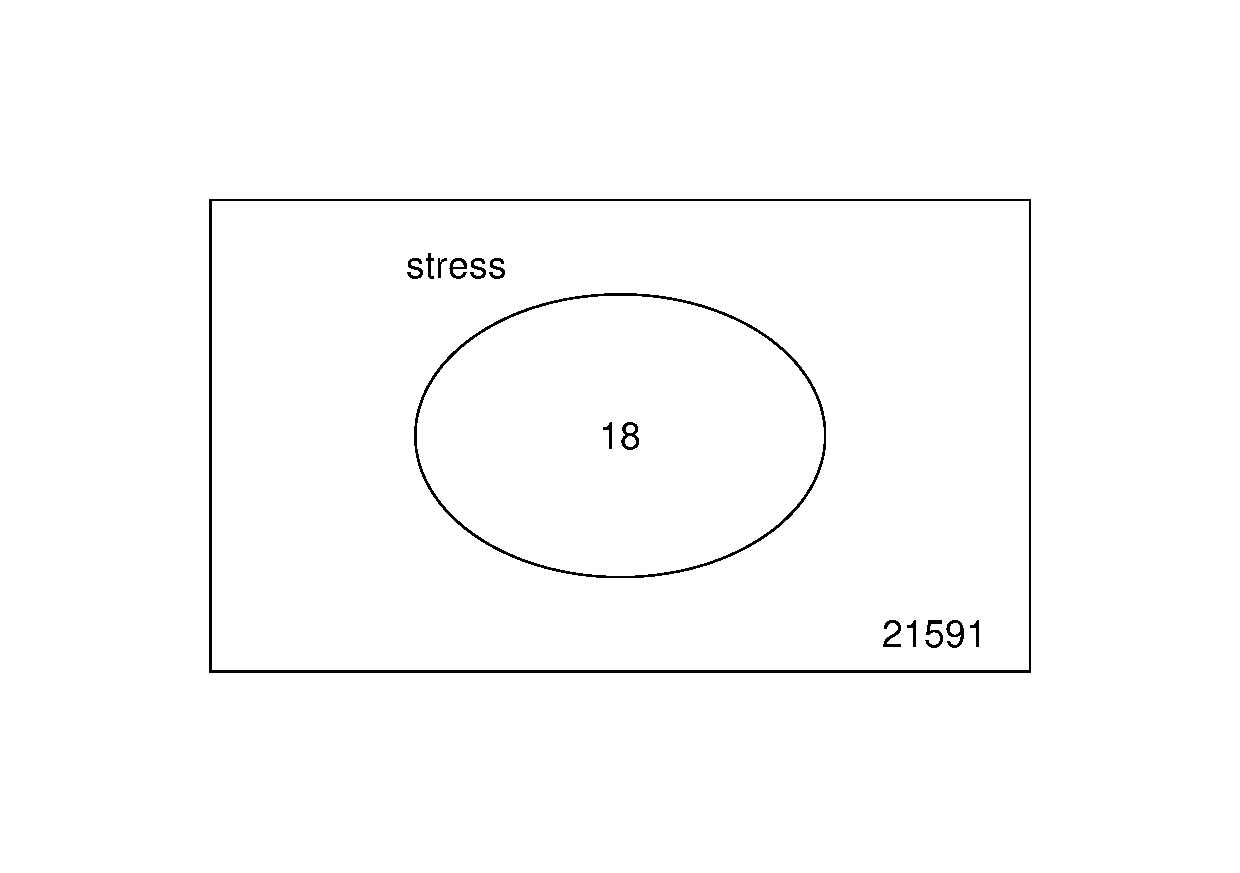
\includegraphics[width=\textwidth, height=4cm]{../../results/plots-and-tables/4.2-DEG-Venn-Diagr-Oryza_sativa}
    \end{subfigure}
\end{figure}



\begin{figure}[htbp]
    \caption{Heatmap of the DEGs - O. nivara}
    \label{fig:4.4-DEG-Heatmap-Oryza_nivara}
    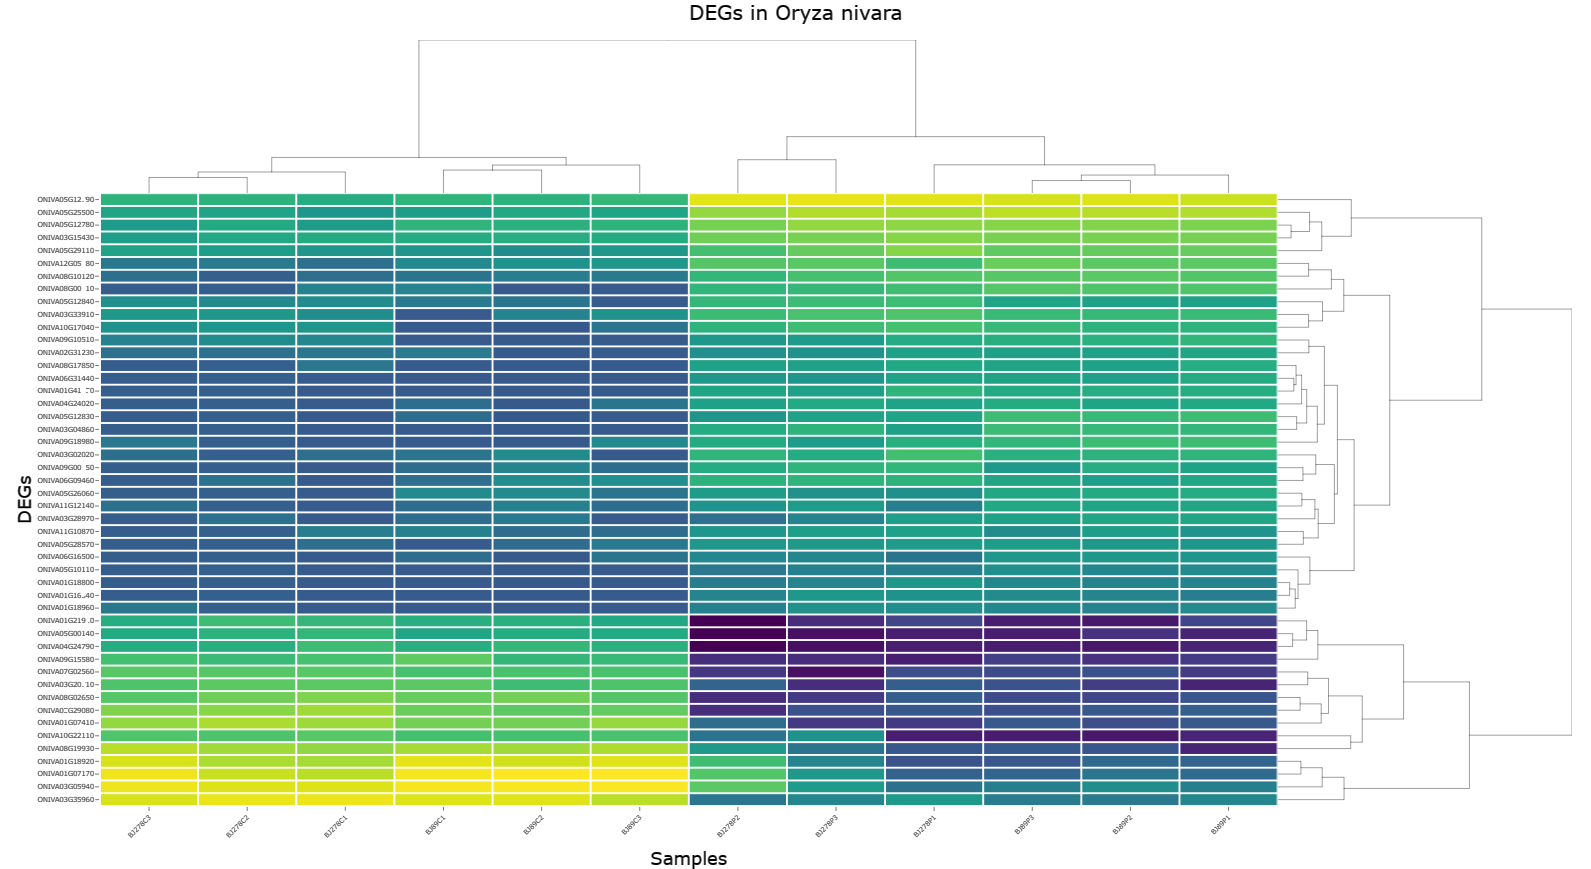
\includegraphics[width=\textwidth]{../../results/plots-and-tables/4.4-DEG-Heatmap-Oryza_nivara}
\end{figure}

\begin{figure}[htbp]
    \caption{Heatmap of the DEGs - O. sativa}
    \label{fig:4.4-DEG-Heatmap-Oryza_sativa}
    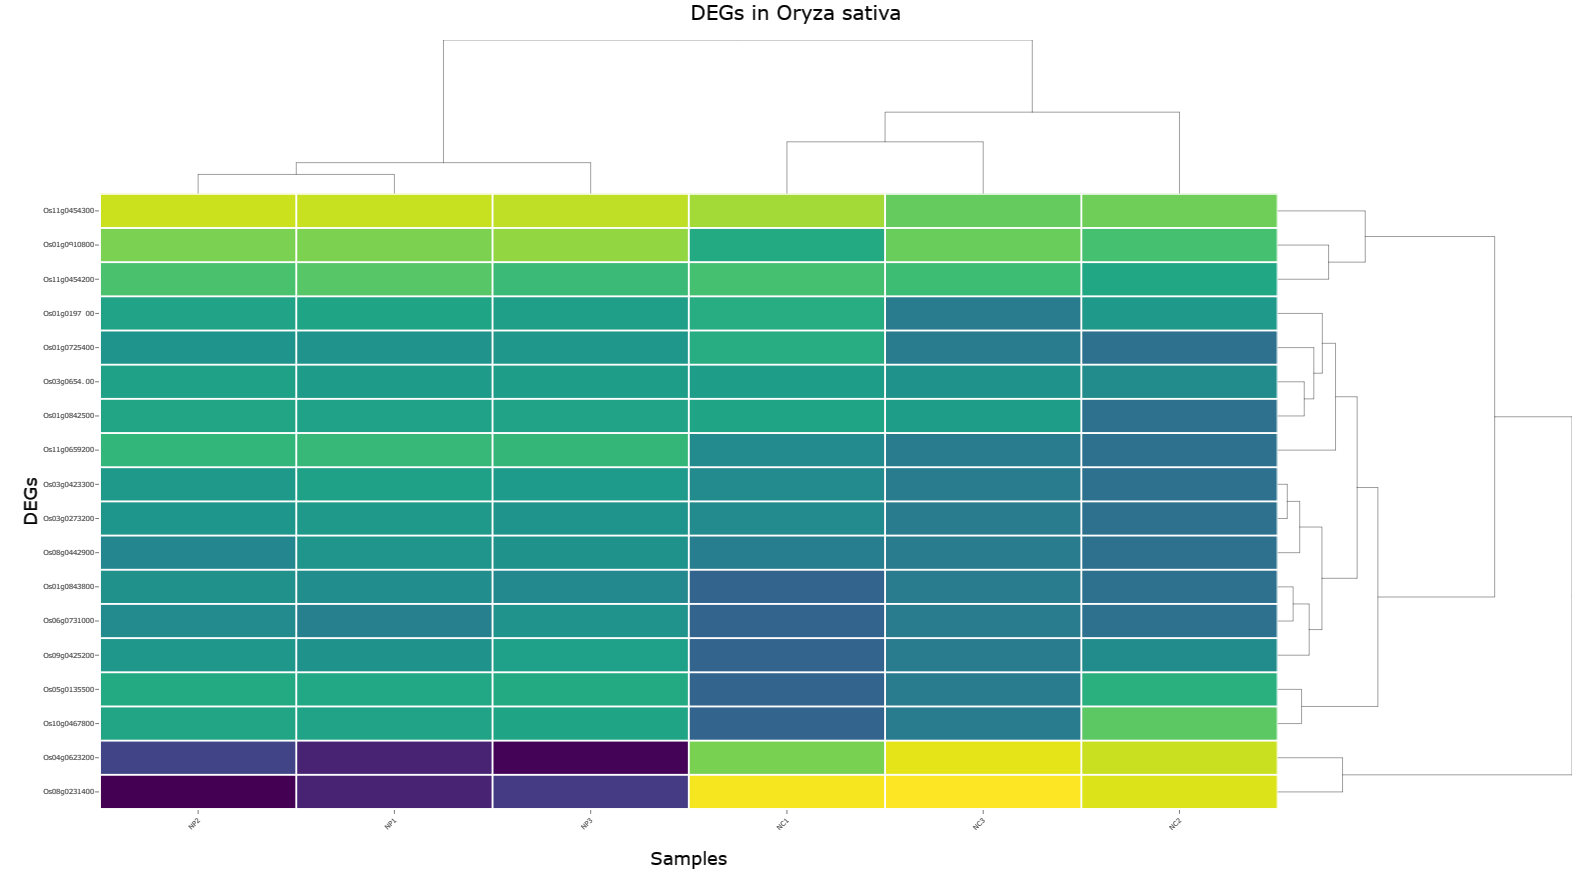
\includegraphics[width=\textwidth]{../../results/plots-and-tables/4.4-DEG-Heatmap-Oryza_sativa}
\end{figure}



TODO: Discuss the identified differentially expressed genes and their potential biological significance.

\subsection{Functional enrichment analysis}



\begin{figure}[htbp]
    \caption{Manhattan plot with the first 10 top-ranked GO terms highlighted - O. nivara}
    \label{fig:5.2-Gost-Plot-Oryza_nivara}
    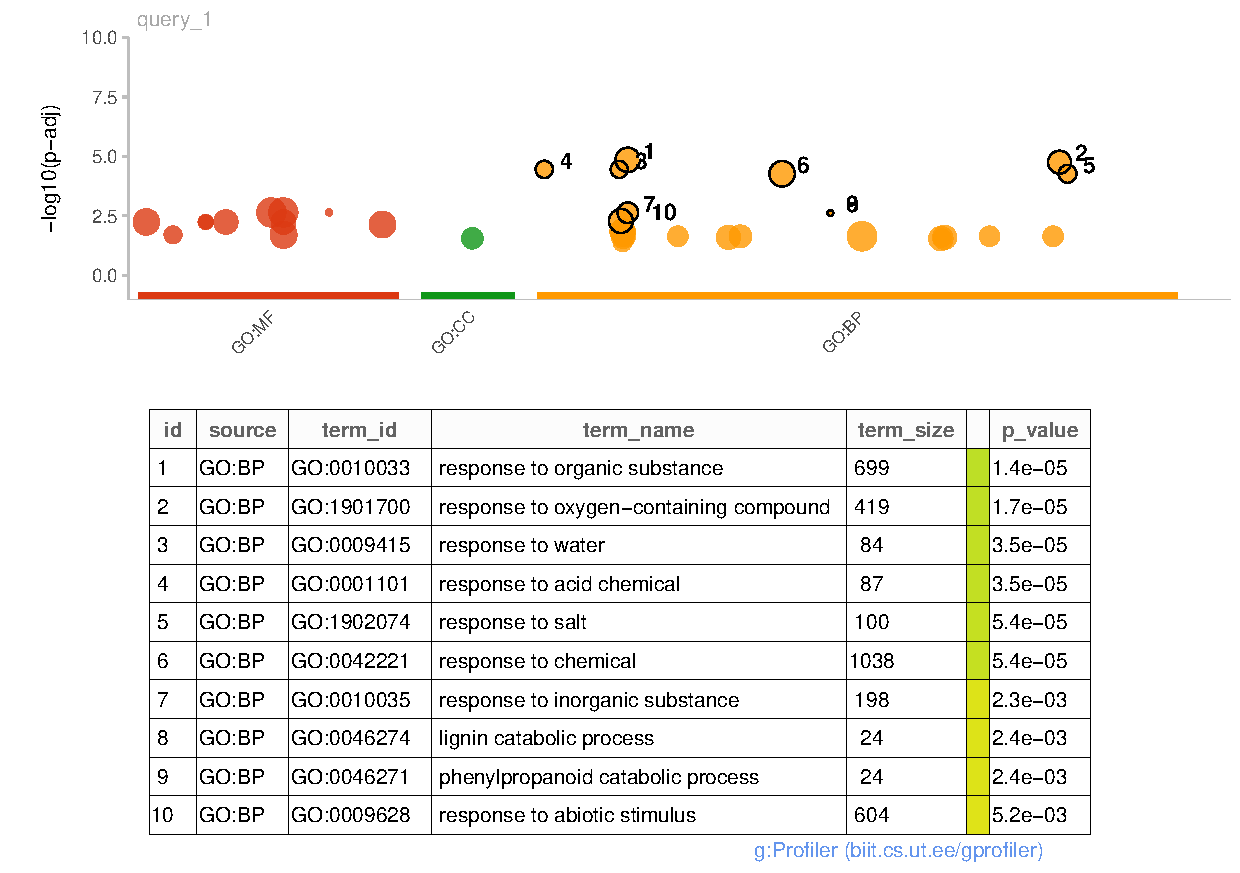
\includegraphics[width=\textwidth]{../../results/plots-and-tables/5.2-Gost-Plot-Oryza_nivara}
\end{figure}

\begin{figure}[htbp]
    \caption{Manhattan plot with the first 10 top-ranked GO terms highlighted - O. sativa}
    \label{fig:5.2-Gost-Plot-Oryza_sativa}
    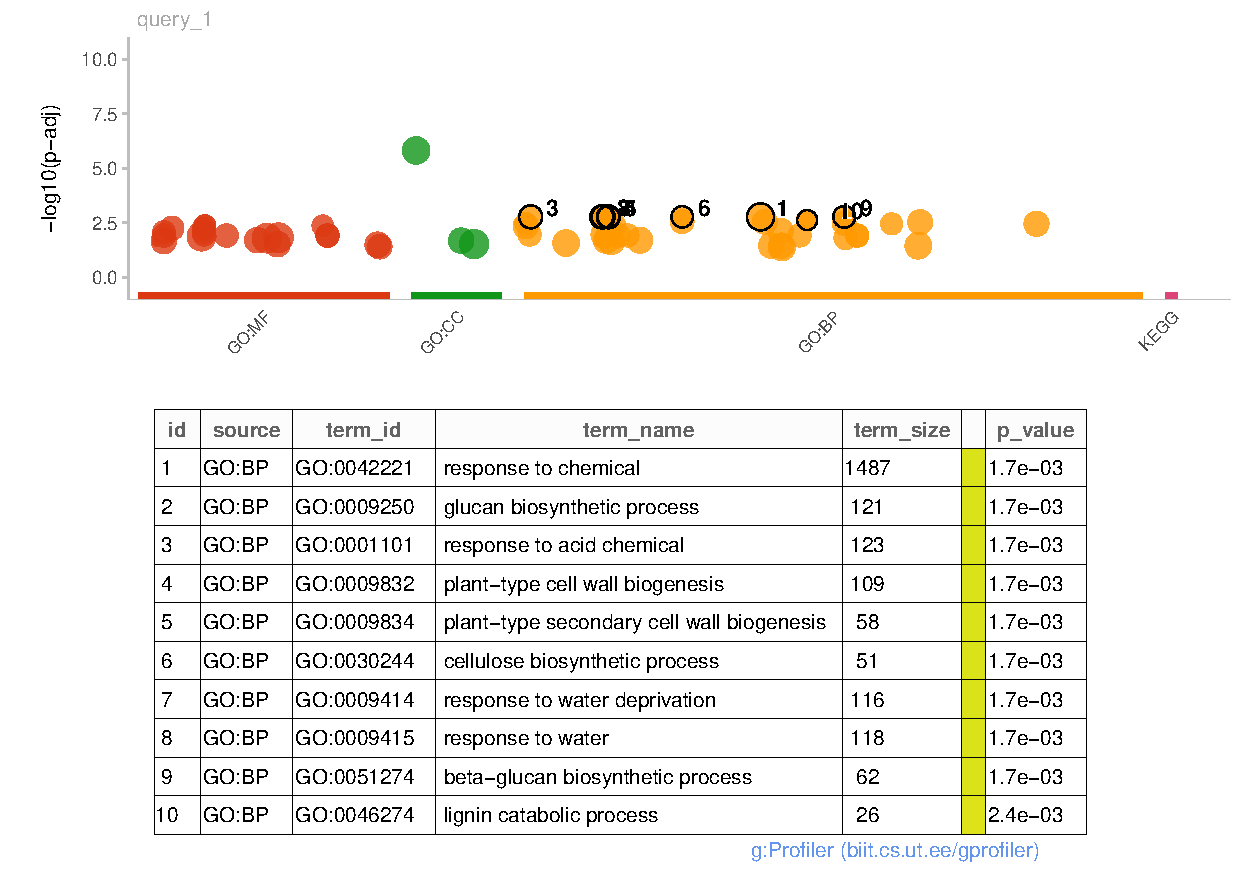
\includegraphics[width=\textwidth]{../../results/plots-and-tables/5.2-Gost-Plot-Oryza_sativa}
\end{figure}



TODO: Present the results of the functional enrichment analysis, highlighting the enriched functional categories.